\documentclass[12pt, french, latin.medieval, a4paper]{report}
% package de langues 
\usepackage[french]{babel}
\usepackage[utf8]{inputenc}
\usepackage[T1]{fontenc}

% package pour référence de liens sur pdf 
\usepackage[pdftex]{hyperref} % liens
\usepackage{lastpage} % numéro de page
\usepackage{caption}

% package de formes de document 
\usepackage[left=2.5cm,
              right=2.5cm,
              top=2.5cm,
              bottom=2.5cm
             ]{geometry}
% pour les tableaux 
\usepackage{array,multirow,makecell} 
\newcolumntype{R}[1]{>{\raggedleft\arraybackslash }b{#1}}
\newcolumntype{L}[1]{>{\raggedright\arraybackslash }b{#1}}
\newcolumntype{C}[1]{>{\centering\arraybackslash }b{#1}}

% package pour la page de couverture 
\usepackage{graphicx}
\usepackage[cyr]{aeguill}
\usepackage{fancyheadings}
\usepackage{amsmath}
\usepackage{amsfonts}
\usepackage{amssymb}
\usepackage{geometry}
\usepackage{eso-pic}
\usepackage{tikz}
\usetikzlibrary{calc}


% nouvelle commande pour la forme 
%\fancyhf[OFC]{\thepage / \pageref{LastPage}}
\rfoot{\thepage / \pageref{LastPage}}
%\setcounter{tocdepth}{3}

% pakages de couleurs du document
\usepackage{color}
\usepackage{xcolor}


% package pour la chimie
\usepackage[version=4]{mhchem}


% package pour la visualisation du code
\usepackage{listings}
\definecolor{darkWhite}{rgb}{0.94,0.94,0.94}
 
\lstset{
  aboveskip=3mm,
  belowskip=-2mm,
  backgroundcolor=\color{darkWhite},
  basicstyle=\footnotesize,
  breakatwhitespace=false,
  breaklines=true,
  captionpos=b,
  commentstyle=\color{red},
  deletekeywords={...},
  escapeinside={\%*}{*)},
  extendedchars=true,
  framexleftmargin=16pt,
  framextopmargin=3pt,
  framexbottommargin=6pt,
  frame=tb,
  keepspaces=true,
  keywordstyle=\color{blue},
  language=python,
  literate=
  {²}{{\textsuperscript{2}}}1
  {⁴}{{\textsuperscript{4}}}1
  {⁶}{{\textsuperscript{6}}}1
  {⁸}{{\textsuperscript{8}}}1
  {€}{{\euro{}}}1
  {é}{{\'e}}1
  {è}{{\`{e}}}1
  {ê}{{\^{e}}}1
  {ë}{{\¨{e}}}1
  {É}{{\'{E}}}1
  {Ê}{{\^{E}}}1
  {û}{{\^{u}}}1
  {ù}{{\`{u}}}1
  {â}{{\^{a}}}1
  {à}{{\`{a}}}1
  {á}{{\'{a}}}1
  {ã}{{\~{a}}}1
  {Á}{{\'{A}}}1
  {Â}{{\^{A}}}1
  {Ã}{{\~{A}}}1
  {ç}{{\c{c}}}1
  {Ç}{{\c{C}}}1
  {õ}{{\~{o}}}1
  {ó}{{\'{o}}}1
  {ô}{{\^{o}}}1
  {Õ}{{\~{O}}}1
  {Ó}{{\'{O}}}1
  {Ô}{{\^{O}}}1
  {î}{{\^{i}}}1
  {Î}{{\^{I}}}1
  {í}{{\'{i}}}1
  {Í}{{\~{Í}}}1,
  morekeywords={*,...},
  numbers=left,
  numbersep=10pt,
  numberstyle=\tiny\color{black},
  rulecolor=\color{black},
  showspaces=false,
  showstringspaces=false,
  showtabs=false,
  stepnumber=1,
  stringstyle=\color{gray},
  tabsize=4,
  title=\lstname,
}

%package pour les algorithmes
\usepackage{algorithm}
\usepackage{algorithmic}
\usepackage{amsmath}

% package pour les tableaux
\usepackage{longtable}
\usepackage{booktabs}

% package pour les figures 
\usepackage{subcaption}

% package de reférencement
% \usepackage[backend=biber,safeinputenc, sorting=none]{biblatex}

% mettre la bibliographie dans la table de matières
%\usepackage[nottoc, notlof, notlot]{tocbibind}
\include{page_couverture.tex}


\author{MBE MBE MINDJANA LOIC HENRI}
\title{GNPS et MDByTE}

\begin{document}
    
    \pagecouverture
    {Outils bio-informatiques GNPS et MADByTE}
    {}
    
    \tableofcontents
    \vspace{20cm}
    % introduction

    \section{Introduction}
    Pour les recherches de découverte issues des produits naturelles dans un pole médicinale, les techniques de spectrométrie de masse et de résonnance magnétique nucléaire sont grandement utilisé pour le procéssus de déréplication, quant à leur capacité à capturer la structure chimique d'un composé ou molécule complexe ou non. Des outils ont été ainsi crées pour réaliser la déréplication en s'appuyant sur le modèle de \textbf{réséau moléculaire}, dont on peut citer \textbf{GNPS} (Global Natural Product Social) s'appuyant sur la spectrométrie de masse et \textbf{MADByTE} (Metabolomics And Dereplication By Two-dimensional Experiments) s'appuyant sur la spectrométrie par résonnace magnétique nucléaire. Qu'est ce que GNPS et MADByTE d'un point de vue scientifique et technologique, quelle est le workflow de GNPS et de MADByTE, qu'est-ce-qu'ils prenent en entrée et retourne en sortie ? Dans les lignes qui suivent nous essayerons de repondre a ces questions, en présentant d'une part GNPS et d'autre part MADBYTE. 

    % contexte globale

    \section{Contexte Globale}
    Pour réaliser la déréplication des produits naturelle de nos jours, on utilise deux outils, à savoir GNPS qui permet d'obtenir sur la base d'un ensemble de spectres tandem $MS/MS$ ou encore $MS^{2}$  (Mass Spectrometry) d'obtenir un réseau moléculaire et MADByTE par contre permet de le faire mais sur la base de spectres 2D $RMN$ (Raisonnace Magnétique Nucléaire). Comment combiner les deux approches ?, est la question a laquelle nous devons repondre pour pouvoir les combiner afin d'améliorer le qualité des réseaux moléculaires finaux. premierement nous devront comprendre les approches de mise en réseau moléculaire de GNPS et MADByTE, et ensuite y faire si possible des remarques pour avoir un point de départ d'idée pour la combinaison.

    % outil gnps
    
    \section{Outil GNPS}
   
   % problématique, probleme et solution
   \subsection{Problématique, problème et solution}
    L'outil GNPS est la résultante de l'article \cite{wang2016sharing} qui attaque la problématique de partage et d'extraction de connaissance d'une grande plage de données spectrales MS/MS dans le but d'éffectuer la déréplication en utilisant comme modèle final d'interprétation les réseaux moléculaires. Il c'est a dire l'article se base sur le fait que la capture d'information structurale faite actuellement ( selon son temps) d'un ne se base pas sur une grande quantité de spectre et deux n'utilise pas des modeles d'interprétation capturant vraiment l'espace chimique d'une grande quantité de spectre. Il a ainsi conduit à une documentation technique disponible \href{https://github.com/CCMS-UCSD/GNPSDocumentation/tree/notebooks-docs}{ici}. 

    % présentation concrete de GNPS suivant l'article 
    \subsection{Présentation de GNPS suivant l'article}
    
    \subsubsection{ Base publique GNPS, dépots et librairies spectrales publiques}
    
    IL c'est a dire GNPS, s'appuie sur une banque spectrale qui est mis a jour soit par des résultantes d'expériences validées par des paires, soit par des échanges rigoureuses entre utilisateurs de GNPS; également il communique avec les librairies publiques de référence \ref{fig:gnps1} tel que 
    \textbf{MassBank}\cite{horai2010massbank}(Japon, Europe, Amerique du nord), 
    \textbf{ReSpect}\cite{sawada2012riken}, 
    \textbf{BDMH}, \href{https://www.nist.gov/srd/nist-standard-reference-database-1a}{\textbf{NIST}} accéssible en lecture, et des dépots publiques telque 
    \href{https://metaspace2020.eu/}{\textbf{MetaSpace}}. 

    \begin{figure}
        \begin{center}
            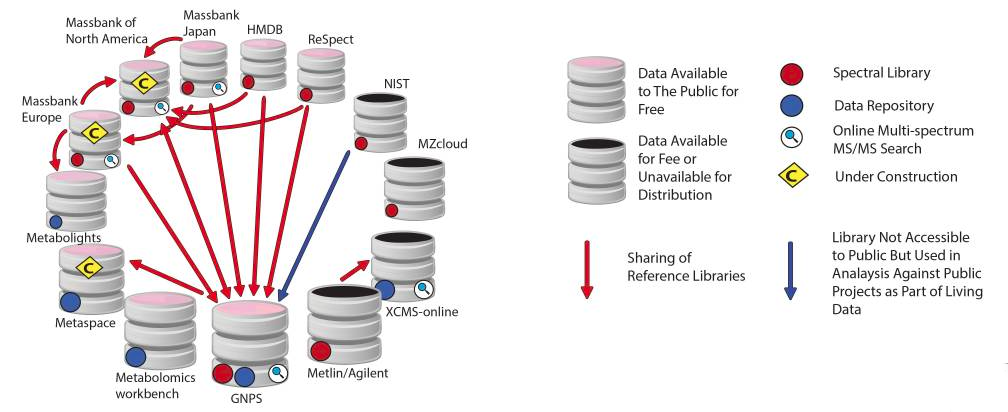
\includegraphics[width = \textwidth]{Images/GNPS10.png}
        \end{center}
        \caption{communication entre la base GNPS et autres bases}
        \label{fig:gnps1}
    \end{figure}

    \subsubsection{Workflow de GNPS}
    Le workflow de GNPS \ref{fig:gnps3} est présent sur la figure suivante: 
    \begin{enumerate}
        \item En entrée on a les spectres MS/MS issus d'une expérience précise
        \item On effectue parallement :
            \begin{itemize}
                \item la recherche de ces dernières dans la banque GNPS afin de savoir s'il sont des molécules \textbf{identifiées}, \textbf{une molécule identifiée} étant une molécule qui possède au moins avec une molécule de la base GNPS \textbf{un score de cosinus de simmilarité strictement supérieur à 0.7}, il faut noter que la cosinus de simmilarité est décrit par la formule suivante 
                    \begin{equation}
                        \cos(sp1, sp2) = \frac{<sp1, sp2>}{||sp1||\times||sp2||}\ avec\ \cos(sp1, sp2) \in [-1, 1]
                    \end{equation}
                Et que si $\cos(sp1, sp2) = 1$ alors on a une correspondante directe. 
                
                on ajoute ainsi les métadonnées liés aux spectres à savoir l'activité biologique, l'ion précurseur, le nom de la molécule, l'origine du spectre ... etc
                \item l'alignement spectrale de ces spectres s'appuyant sur un algorithme qui permet sur la base de leur simmilarité de cosinus de construire un réseau moléculaire telque les noeuds proches indique une simmilarité proche \ref{fig:gnps2}
                
            \end{itemize}
            
        \item on ajoute aux noeuds du réseau les métadonneés liées aux spectres correspondantes, ce qui constitue le réseau moléculaire finale
    \end{enumerate}
    \begin{figure}
        \begin{center}
            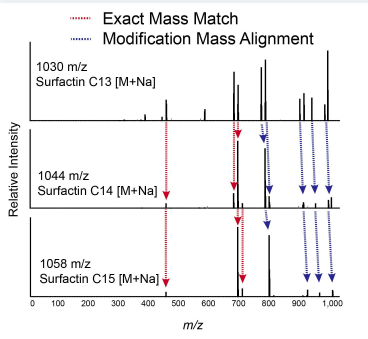
\includegraphics[scale= 0.8]{Images/GNPS8.png}
        \end{center}
        \caption{Alignement spectrale du surfacin C13[M+Na], C14[M+Na] et C15[M+Na]}
        \label{fig:gnps2}
    \end{figure}
    
    On dégage ainsi un certains nombre de notions
    \begin{itemize}
        \item \textbf{molécule identifiée}: molécule qui possède au moins avec une molécule de la base GNPS $\cos(sp1, sp2) > 0.7$
        \item \textbf{molécule putative}: molécule non identifiée, mais voisin directe de ceux identifiées
        
        \item \textbf{réseau identifié}: sous réseau du réseau moléculaire, qui ne possède que des noeuds identifiés

        \item \textbf{réseau non identifié}: sous réseau du réseau moléculaire, qui ne possède que des noeuds non identifiés

        \item \textbf{réseau exploratoire}: réseau construit sur la base de molécule identifiées sous la base de score de cosinus $\cos(sp1, sp2) > 0.63$
    \end{itemize}

\subsubsection{Evaluation}
    L'utilisation de la base publique GNPS de partage publique, a permis d'avoir une capture plus grande de l'espace chimique contenu dans les spectres MS/MS des utilisateurs de GNPS rendus publiques et des spectres MS/MS des libraries publiques. \ref{fig:gnps4}
    
    \begin{figure}
        \begin{center}
            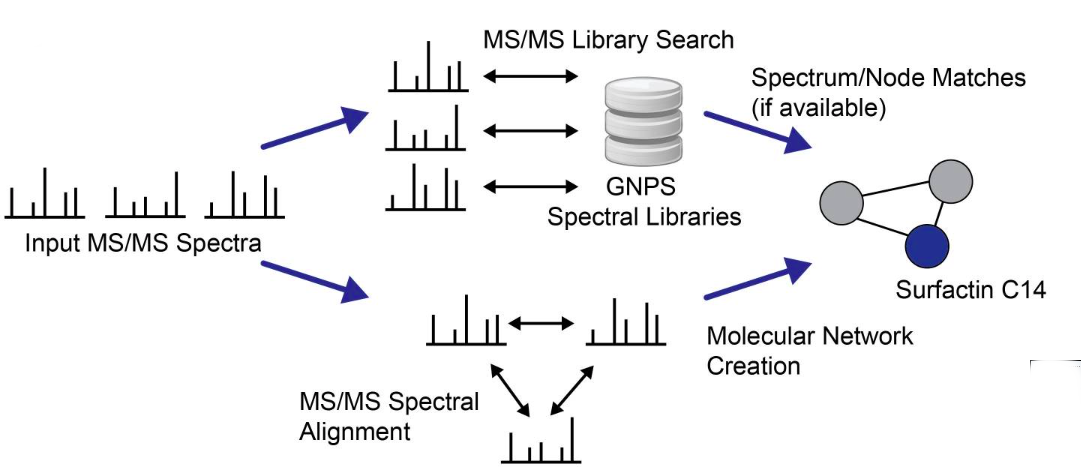
\includegraphics[width = \textwidth]{Images/GNPS4.png}
        \end{center}
        \caption{Workflow de déréplication GNPS}
        \label{fig:gnps3}
    \end{figure}

    Et surtout vue que les réseaux moléculaires sont obtenus sur la base de la librairie GNPS qui est sans sesse croissance, on aura ainsi progréssivement des réseaux moléculaires de meilleure qualité dans le sens qu'on pourrait avoir de plus en plus de molécules identifiés.

    \begin{figure}
        \begin{center}
            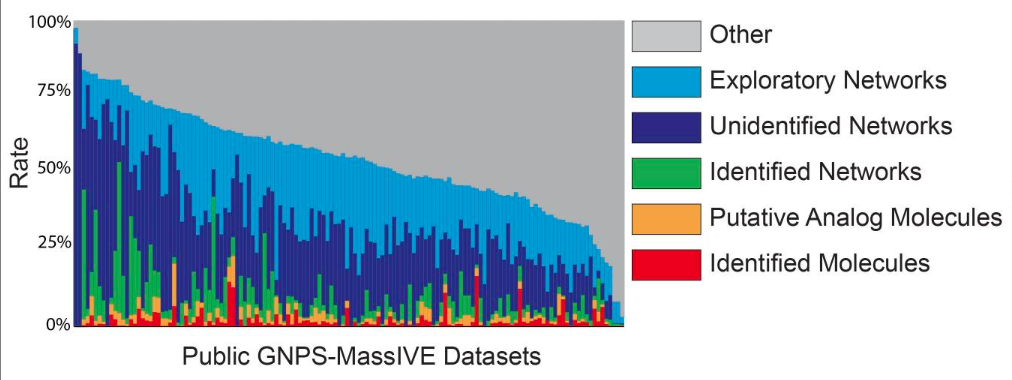
\includegraphics[width = \textwidth]{Images/GNPS3.png}
        \end{center}
        \caption{Graphique d'évaluation de GNPS apres 4 ans de sa création: Ici on évalue les taux des molécules identifiées, putatives, réseaux identifiés, non identifiés, réseaux d'exploration et autres sur les datasets de spectres massives publiques de GNPS }
        \label{fig:gnps4}
    \end{figure}
    
    GNPS a permit ainsi la découverte de la famille molécule \textbf{stenothricine}  en utilisation comme spectre d'entrée les extraits de \textbf{S. roseosporus  NRRL 15998 } (stenothricine) et \textbf{Streptomyces sp. DSM5940} \ref{fig:gnps5}(stenothricine); on a ainsi pu savoir qu'il y avait qu'un décalage de spectre de -4Da (Da étant l'unité de masse atomique) suivant l'axe m/z entre les spectres de la stenothricine issus de l'expérience et celui contenu dans la base GNPS \ref{fig:gnps6}.
    
    \begin{figure}
        \begin{center}
            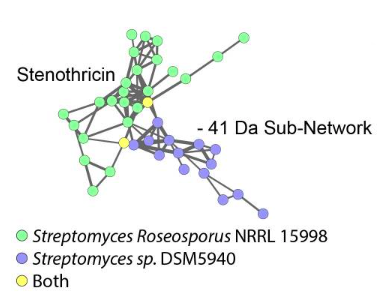
\includegraphics[width = \textwidth]{Images/GNPS6.png}
        \end{center}
        \caption{Réseau moléculaires issues des spectres d'extraits de \textbf{S. roseosporus  NRRL 15998 } (en vert) et  \textbf{Streptomyces sp. DSM5940} (en bleu)}
        \label{fig:gnps5}
    \end{figure}

    \begin{figure}
        \begin{center}
            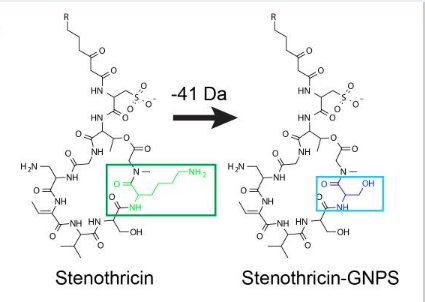
\includegraphics[width = \textwidth]{Images/GNPS1.png}
        \end{center}
        \caption{Visualisation de la stenothricine de l'expérience et de celui contenu dans la base GNPS}
        \label{fig:gnps6}
    \end{figure}
    
    \begin{figure}
        \begin{center}
            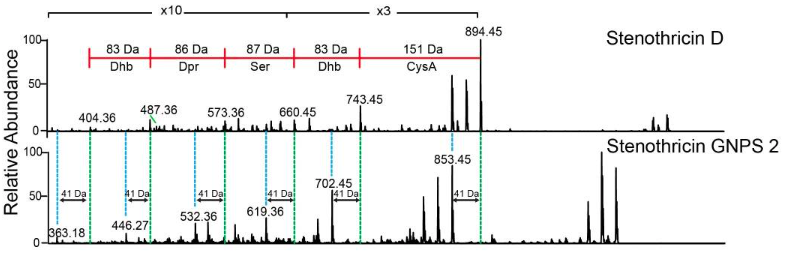
\includegraphics[width = \textwidth]{Images/GNPS2.png}
        \end{center}
        \caption{Visualisation des spectres de la stenothricine de l'expérience et de celui contenu dans la base GNPS}
        \label{fig:gnps7}
    \end{figure}

    % outil MADByTE
   
    \section{Outil MADByTE}
   
   % problématique, probleme et solution
   \subsection{Problématique, problème et solution}
    L'outil MADByTE est la solution de l'article \cite{egan2021development} qui attaque la problematique d'annotation de mixtures(mélanges) complexes de produits naturelles en utilisant la spectrométrie 2D-RMN. Pour resoudre cette problematique des solutions ont été crées mais toutes n'étaient pas suffisamment simple pour caractériser l'espace chimique dans les spectres 2D-RMN, c'est a dire n'étaient pas suffisament simple pour avoir des résultats aisement interprétables pour l'annotation ou simplement l'hierarchisation des spectres 2D-RMN ce qui pourrait ètre utile pour la déréplication. cette solution a été réalisé et mis à la disposition du publique sur le dépot git \href{https://github.com/liningtonlab/madbyte}{MADByTE}. 

    % présentation concrete de MADByTE suivant l'article 
    \subsection{Présentation de MADByTE suivant l'article }

    \subsubsection{Introduction}
    Sachant que la spectrométrie de masse a un incnvénient dépendant de la qualité de l'ionisation, du fait qu'une "mauvaise ionisation" conduira à la non détection de certains radicaux et à une introduction de bruits dans les spectres; la spectrométrie RMN a été proposé comme complément à la spectrométrie de masse car plus stable du fait qu'on capture les intensités des résonnances des nucléides par fréquence. Il faut aussi noter que la spectrométrie RMN permet d'obtenir un équilibre entre la qualité ou encore résolution des spectres et leur temps d'aquisition, comparée à la spectrométrie de masse dont les spectres obtenus contiennent généralement du bruit et sont obtenus en un temps plus élévée. 

    Afin de répondre à la problématique d'annotation de mélanges complexes de produits naturelles, suivant les problèmes des solutions existantes recensés, MADByTE a été crée.
    Il utilise un réseau de simmilarité chimique pour:
    \begin{itemize}
        \item la déréplication "d'échafaudages" de composés connus
        \item l'hierachisation des métabolites 
    \end{itemize}

    MADByTE \ref{fig:madbyte1} s'est portée sur deux spectrométries réalisées séparement (pour réduire les risques de bruit), la spectrommétrie 2D-RMN \textbf{HSQC} (Heteronuclear single quantum coherence spectroscopy) s'appuyant sur la connectivité $\ce{^{1}_{}H - ^{13}_{}C}$  et \textbf{TOCSY} (Total Correlation Spectroscopy) s'appuyant plutot sur la connectivité ou encore le couplage $\ce{^{1}_{}H - ^{1}_{}H}$ ; ces dernières permettant de définir les structures discrètes présentent dans chaque échantillon de mélanges complexes. 

    \begin{figure}
        \centering
        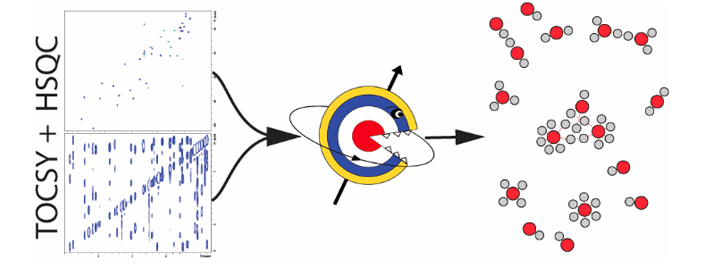
\includegraphics[width=\textwidth]{Images/MADByTE1.png}
        \caption{résumé graphique de MADByTE}
        \label{fig:madbyte1}
    \end{figure}

    Ainsi en entrée, on a les couples de spectres TOCSY et HSQC d'un ensemble de molécules ou de composés, et en sortie on a un ensemble réseau de simmilarités capturant les "simmilarités" des systèmes de "spins" (système de caractéristiques magnétiques des atomes ciblés ) des composés contenus dans leurs couples de spectres.

    \subsubsection{Workflow de MADByTE}
    le workflow de MADByTE \ref{fig:madbyte3} pour obtenir le réseau de simmilarité est le suivant:
    \begin{enumerate}
        \item \textbf{aquisition des données spectrales HSQC et TOCSY}: 
        
        cette aquisition est réalisée par des expériences physico-chimiques des composés qui neccéssite l'intervention des experts
        \item \textbf{selection des pics de HSQC et TOCSY des composés} :
        
        cette étape constitue une étape de prétraitement des spectres HSQC et TOCSY qui passent par les étapes suivantes:
        \begin{enumerate}
            \item suppréssion des pics des solvants et d'eau: 
            
            cela ce fait à bande des déplacements chimiques de $\pm2ppm$ pour la dimension $\ce{^{1}_{}H}$ (la dimension $\ce{^{1}_{}H}$ car dans les solvants telque DMSO-d6 et méthanol-d4, les pics d'hydrogène $\ce{^{1}_{}H}$ sont grandement plus présents) 
            
            \item suppréssion des pics invalides de spectres HSQC obtenus : 
            
            les pics invalides sont caractérisés par les déplacements chimiques sur les dimensions $\ce{^{1}_{}H}$ et $\ce{^{13}_{}C}$ se trouvent sur le tableau \ref{tab:madbyte1} 
            \begin{center}
                \begin{tabular}{|C{2cm}|C{1cm}|}
                    \hline $\ce{^{1}_{}H}$  & $\ce{^{13}_{}C}$ \\
                    \hline  > 7 ppm & < 50 ppm\\
                    \hline  < 7 ppm & > 170 ppm\\
                    \hline  < 2.4 ppm & > 100 ppm\\
                    \hline 
                \end{tabular}
                \captionof{table}{tableau de déplacements chimiques invalides des spectres HSQC}
                \label{tab:madbyte1}
            \end{center}

            \item suppréssion des pics invalides des spectres TOCSY 
            les pics invalides sont ceux issus des déplacements chimiques des dimensions 
            $\ce{^{1}_{}H}$ $\leq$ 2.5 ppm 

            \item symétrisation des spectres TOCSY obtenus : 
            
            Les données TOCSY sont symétrisées en corrigeant les déplacements chimiques f1(dimension $\ce{^{1}_{}H}$ de plus faible résolution) par rapport aux valeurs f2 (dimension $\ce{^{1}_{}H}$ de plus haute résolution) correspondantes, on tient compte des erreurs de déplacements suivant les dimensions 

            \item croisement des couples de spectres HSQC et TOCSY : 
            
            la liste des signaux TOCSY est comparée à la liste des pics HSQC dans la dimension $\ce{^{1}_{}H}$, et les signaux TOCSY n'ayant pas de correspondance avec les signaux HSQC correspondants sont supprimés, et on tient compte des erreurs de déplacements suivant les dimensions 
            
        \end{enumerate}
        L'érreur pour H est 0.05 ppm et pour C est 0.40 ppm
        \item \textbf{création des caractéristiques des systèmes de spins des composés} :
        
        Les caractéristiques des systèmes de spin pour les échantillons individuels sont créées en générant un graphe dirigé à partir de chaque tableau de pics représentant le spectre TOCSY obtenu, où les noeuds représentent les signaux $\ce{^{1}_{}H}$ dans le spectre TOCSY, et les arêtes représentent les pics croisés TOCSY entre les signaux $\ce{^{1}_{}H}$. les noeuds ne contenant qu'une seule arete sont supprimés. De même, les arêtes entre les noeuds sont supprimées si elles ne sont pas réciproques \ref{fig:madbyte2} (c'est-à-dire si elles ne sont pas observées des deux côtés de la diagonale du spectre TOCSY).

        \begin{figure}
            \centering
            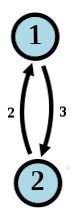
\includegraphics{Images/madbyte2.png}
            \caption{Arètes réciproques: les arètes 2 et 3 sont des arètes réciproques}
            \label{fig:madbyte2}
        \end{figure}
        
        \textbf{En gros une caractéristique du système de spin est une réprésentation sous forme de graphe d'un spectre TOCSY symétrisé et croisé avec un spectre HSQC correspondant suivant la dimension $\ce{^{1}_{}H}$; ce graphe pouvant toujours etre vu comme un tableau }.


        \item \textbf{calcul d'une matrice de corrélation de ces caractéristiques} [partie à vérifier]: utilisé pour obtenir les scores de ressemblance en ces caractéristiques.

        Le score de ressemblance entre les graphes A et B de deux caractéristiques de spins représentant des spectres TOCSY et HSQC obtenues à la fin de l'étape 3, est obtenu de la façon suivante :
        $$ score\ ressemblance\ (A,B) = \frac{nombre\ de couples (\ce{^{1}_{}H},\ce{^{13}_{}C}) \ identiques\ de\ A\ et\ de\ B}{nombre\ total\ de\ couples (\ce{^{1}_{}H},\ce{^{13}_{}C}) \ correspondantes\ de\ A\ et\ de\ B}$$
        Les couples sont identiques au sens où ils sont correspondants , avec les memes valeurs de pics.

        on considère que deux échantillons sont simmilaires si et seulement si leur score de simmilarité dépassent un seuil défini par l'utilisateur (par défaut égale à 0.5)
        
        \item \textbf{construction du réseau de simmilarité} :
        
        Le réseau est obtenu comme suit:
        \begin{enumerate}
            \item  pour chaque échantillon on a d'abord un noeud équivalent qui est reliés à ses noeuds réprésentants les déplacements chimiques valides $\ce{^{1}_{}H}$ qui sont les noeuds du système de spin
            \item  pour chaque paire d'échantillons simmilaires; les noeuds des caractéristiques de spin conduisant la simmilarité sont reliés entre eux, on parle de \textbf{réseau d'association complèt}.
        Afin d'éviter les encombrements des noeuds non utilisés pour représenter la simmilarité entre les échantillons, on les supprime, on parle donc de \textbf{réseau d'association}, et vue que les noeuds de simmilarités sont identiques entre paires d'échantillons on les fusionent et lç on parle de \textbf{réseau d'association hybride}
        \end{enumerate}
       
    \end{enumerate}

    \begin{figure}
        \centering
        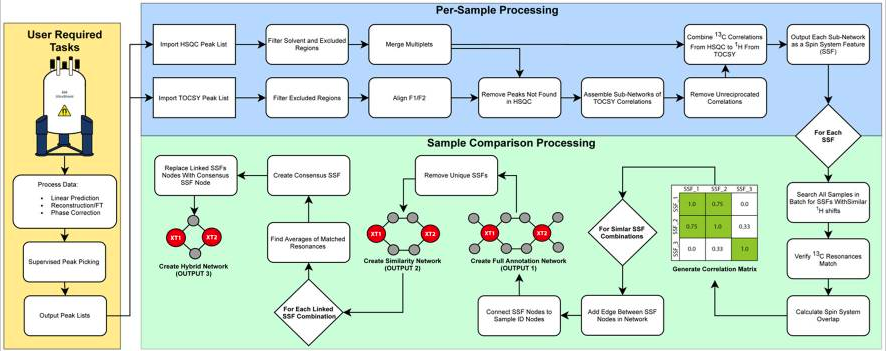
\includegraphics[width=\textwidth]{Images/madbyte3.png}
        \caption{Workflow de MADByTE}
        \label{fig:madbyte3}
    \end{figure}


    \subsubsection{Evaluation}

    Pour tester l'efficacité de la plate-forme de regroupement des classes de composés, les auteurs ont acquis un ensemble de données d'apprentissage comprenant les spectres TOCSY et HSQC pour 17 produits naturels et analogues de produits naturels disponibles dans le commerce . Des caractéristiques sélectionnées du réseau d'association complet résultant sont présentées dansfigure 3(le réseau complet est disponible dans les informations complémentaires comme Figure S5 ). Le réseau d'association complet \ref{fig:madbyte4} contenait un sous-groupe (groupe central) contenant trois composés de référence. Un examen plus approfondi de ce sous-réseau a révélé la présence des molécules apparentés azithromycine ( 3 ), érythromycine ( 4 ) roxithromycine ( 5 ). on as aussi deux autres ensembles de composés correspondants, notamment chloramphénicol ( 1 )/ thiamphénicol ( 2 ) et épirubicine ( 6 )/ daunomycine ( 7 ).

    \begin{figure}
        \centering
        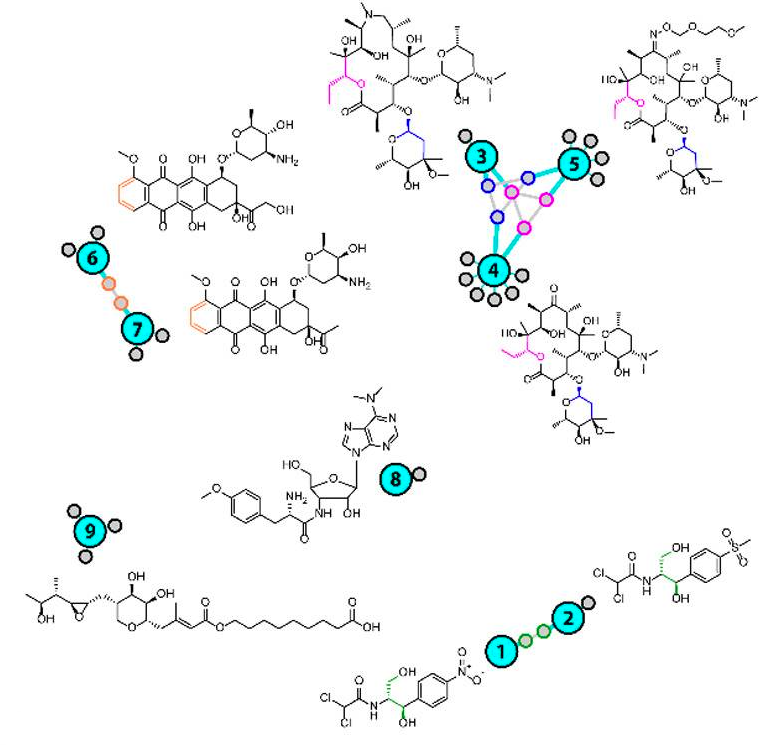
\includegraphics[width=\textwidth]{Images/madbyte4.png}
        \caption{réseau d'association complet pour l'hierachisation de composés connus}
        \label{fig:madbyte4}
    \end{figure}

    Pour évaluer la capacité de la plateforme à identifier des métabolites dans des mélanges complexes, un ensemble de 9 échantillons dopés de préfraction a été préparé, sur la base de composé de réfférence \ref{tab:madbyte2}. 
    \begin{center}
        \begin{tabular}[width=\textwidth]{|C{5cm}|C{3cm}|C{4cm}|C{2cm}|}
            \hline nom des échantillon & Extrait de préfaction & composé enrichi (dopé) & Identifiant \ref{fig:madbyte5} \\
            \hline 1526 A SPK & 1526 A & Erythromycine & A\\
            \hline 1526 C SPK & 1526 C & Mupirocine & B\\
            \hline 1526 E SPK & 1526 E & Novobiocine & C\\
            \hline 1726 A SPK & 1726 A & Novobiocine & D\\
            \hline 1726 C SPK & 1726 C & Erythromycine & E\\
            \hline 1726 E SPK & 1726 E & Mupirocine & F\\
            \hline 1814 A SPK & 1814 A & Mupirocine & G\\
            \hline 1814 C SPK & 1814 C & Novobiocine & H\\
            \hline 1814 E SPK & 1814 E & Erythromycine & I\\
            \hline Mupirocin de référence & - & - & 9\\
            \hline Erthromycine de référence & - & - & 4 \\
            \hline Novobiocine de référence & - & - & 10 \\
            \hline 
        \end{tabular}
        \captionof{table}{Tableau des échantillons utilisés pour l'évaluation de MADByTE de la capacité d'identification des métabolites de mélanges complexes}
        \label{tab:madbyte2}
    \end{center}
    \begin{figure}
        \centering
        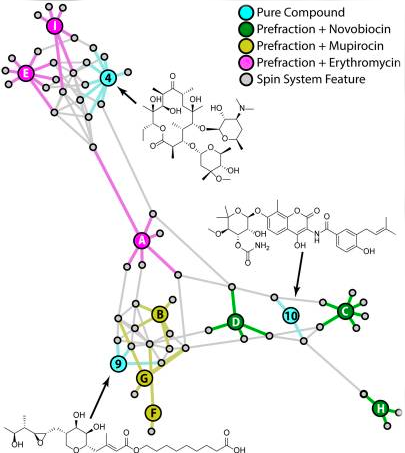
\includegraphics[width=\textwidth]{Images/madbyte5.png}
        \caption{Réseau d'associations complet pour l'évaluation de MADByTE de la capacité d'identification des métabolites de mélanges complexes}
        \label{fig:madbyte5}
    \end{figure}
    Le réseau obtenu, a conduit à dire que MADByTE permettait de le faire pour un grand nombre de fois sur de tel données d'entrée.

    Pour étendre l'évaluation à la déréplication, 85 échantillons de produits naturels microbiens préfractionnés téléchargeable \href{https://doi.org/10.5281 /zenodo.4317721}{ici}, ont été utilisé comme base de déréplication; ces échantillons ont été combinés avec un ensemble de composés purs, le réseau hybride obtenu \ref{fig:madbyte6} a permis de voir que plusieurs préfractions de produits naturels contenaient des caractéristiques de système de spin liées à des composés de référence, suggérant la présence de familles de composés connues dans la bibliothèque d'extraits.

    \begin{figure}
        \centering
        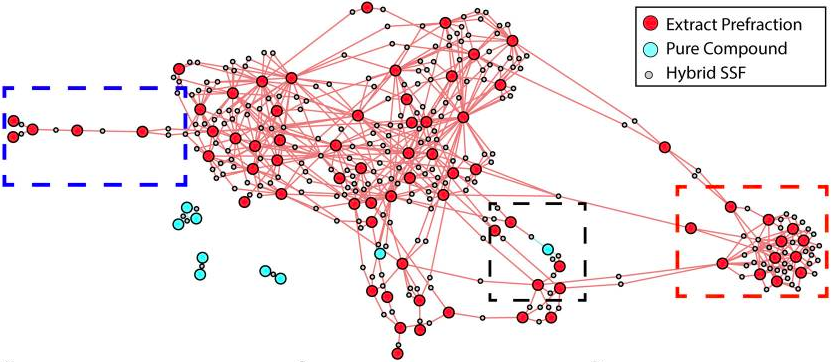
\includegraphics[width=\textwidth]{Images/madbyte6.png}
        \caption{Réseau d'associations complet pour l'évaluation de MADByTE de la déréplication}
        \label{fig:madbyte6}
    \end{figure}

    \subsection{Implémentation suivant les auteurs}

    Afin d'obtenir MADByTE, tel que décrit ci dessus, les auteurs l'on dévéllopé comme un projet logiciel qui a été partagé au public par le biais du dépot \href{https://github.com/liningtonlab/madbyte}{MADByTE}. 

    \subsubsection{Structure du projet}
    MADByTE est un programme en interface graphique, qui a été réalisé en python , par le biais de librairies comme :
    \begin{itemize}
        \item NetworkX : qui permet de visualiser et de manipuler les graphes 
        \item QT5 : qui a permis de mettre sur pied l'UI de l'application 
        \item Pandas : pour pouvoir traiter les sources de données spectrales
        \item numpy : pour facilement réaliser des opérations vectorielles
        \item jotlib : pour pouvoir réaliser des taches en parallèle
        \item pytest : pour les tests automatiques de code python
    \end{itemize}

    \begin{center}
        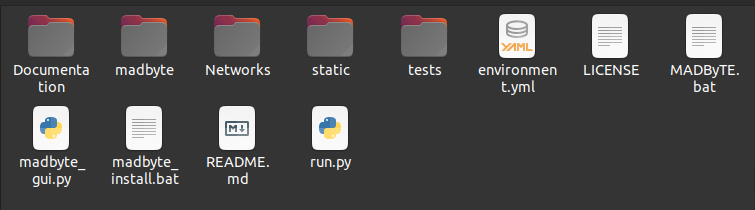
\includegraphics[width = \linewidth]{Images/implementation_MADByTE1.png};
    \end{center}

    On a dans le dépot
    \begin{itemize}
        \item le dossier "Documentation" qui contient de la documentation sur le code
        \item le dossier "madbyte" qui contient les opérations importantes décrite ci dessus 
        \item le dossier "Networks" qui présente 3 exemples simple d'utilisations de réseautage (complet, hybride et simple) par page web
        \item le dossier "static" qui contient les "assets" du programme (icons, image, ...) 
        \item le dossier "test" qui contient les tests automatiques effectuées
        \item les fichiers de "lancement" du programme, la "license MIT" du projet, le "readme" du projet et le fichier "d'environnement" qui contient toutes les librairies à installer avec leur version récommandé. 
    \end{itemize}
    
    \subsubsection{Implémentations des fonctions importantes}

    Algoritme de selection des peaks tocsy et hsqc
\begin{lstlisting}

def tocsy_in_hsqc(tocsy, hsqc, tolerance=0.05, name="MADByTE", inplace=True):
    """Takes TOCSY + HSQC dataframes and removes protons from
    TOCSY not in HSQC

    Args:
        tocsy (pd.DataFrame): TOCSY dataframe
        hsqc (pd.DataFrame): HSQC dataframe
        name (str, optional): Name of sample for logging
        inplace (bool, optional): Apply filtering inplace. Defaults to True.
    """
    hsqc_points = hsqc.H_PPM.values
    bad_points = set()
    for idx, row in tocsy.iterrows():
        if not any([math.isclose(row.Ha, x, abs_tol=tolerance) for x in hsqc_points]):
            logger.debug(f"{name} : TOCSY cleanup {row.Ha} as `Ha` was not found in the HSQC data")
            bad_points.add(idx)
        if not any([math.isclose(row.Hb, x, abs_tol=tolerance) for x in hsqc_points]):
            logger.debug(f"{name} : TOCSY cleanup {row.Hb} as `Hb` was not found in the HSQC data")
            bad_points.add(idx)

    logger.info(f"{name}: There are {len(list(bad_points))} points to remove the the TOCSY peak list that are not in the HSQC")

    # Apply function and return None if inplace=True
    # Otherwise return DF
    return tocsy.drop(bad_points, inplace=inplace)

\end{lstlisting}

Algorithme d'alignement spectrale 

\begin{lstlisting}
    def align_tocsy_hsqc(tocsy, hsqc):
    """Takes TOCSY + HSQC dataframes and aligns TOCSY with HSQC protons

    Args:
        tocsy (pd.DataFrame): TOCSY dataframe
        hsqc (pd.DataFrame): HSQC dataframe
        name (str, optional): Name of sample for logging
    """
    hsqc_points = hsqc.H_PPM.values
    ### Adjusted for analysis of points being re-assigned ###
    try:
        TOCSY_Reassginment_DF = pd.read_csv('TOCSY_Point_assignment.csv',index_col=0)#
    except:
        TOCSY_Reassginment_DF = pd.DataFrame(columns=['TOCSY_point','HSQC_point'])#
    
    for idx, row in tocsy.iterrows():
        # Get closest values
        closest_ha = hsqc_points[np.abs(hsqc_points-row.Ha).argmin()]
        closest_hb = hsqc_points[np.abs(hsqc_points-row.Hb).argmin()]
        # Set closest values
        if not math.isclose(row.Ha, closest_ha, abs_tol=0.001):
            logger.debug(f"{name} : Ha: {row.Ha}, {closest_ha}")
            TOCSY_Reassginment_DF = DF.append({'TOCSY_point':row.Ha,'HSQC_point':closest_ha},ignore_index=True)#
            tocsy.loc[idx, 'Ha'] = closest_ha
        if not math.isclose(row.Hb, closest_hb, abs_tol=0.001):
            logger.debug(f"{name} : Hb: {row.Hb}, {closest_hb}")
            TOCSY_Reassginment_DF = DF.append({'TOCSY_point':row.Hb,'HSQC_point':closest_hb},ignore_index=True)#
            tocsy.loc[idx, 'Hb'] = closest_hb
    # drop duplicates
    tocsy.drop_duplicates(["Ha", "Hb"], inplace=True)
    TOCSY_Reassginment_DF.to_csv('TOCSY_Point_assignment.csv')#

\end{lstlisting}
    
    \section{Remarques}

    Les deux méthodes s'appuient sur des mésures de simmilarité différentes pour construire les réseaux moléculaires ou encore de simmilarité, pour GNPS on utilise le cosinus de simmilarité, et au niveau de MADByTE on utilise tout simplement un taux de ressemblance des caractéristiques du système de spin. On peut dès lors penser que pour combiner les deux solutions on pourrait juste s'appuyer sur une mésure de simmilarité incluant ces deux dernieres simmilarité en attribuant des poids au mésure de simmilarité après normalisation des mésures, ou encore on pourrait plutot pondérer le score de simmilarité avec le taux de simmilarité de spectres TOCSY+HSQC.

    On peut également se rendre compte les spectres au niveau des deux méthodes est obtenus sur la base de techniques de spectrométries entièrement manuel coutant énormement. On peut donc penser à un modèle d'apprentissage automatique qui permettra de générer sur la base d'une réprésentation de la molécule comme SMILES et INCHI d'obtenir des spectres RMN et MS. Est ce vraiment pertinent de le faire? Est la question que nous nous posons.

    De plus les réseaux moléculaires/simmilarités obtenus des deux sont différent  dans le sens où les noeuds pour MADBytE ne représente pas directement le composé sujet de spectrométrie comme dans GNPS mais plutot indiquent les déplacements chimiques valides suivant la dimension $\ce{^{1}_{}H}$ des spectres TOCSY obtenu après croisemnt avec les spectres HSQC. Dans les réseaux de MADByTE la simmilarité ne se visualise pas entre les les échantillons.

    
    \section{Questions}
    On dispose d'un ensemble de questions qui sont les suivantes :
    \begin{itemize}
        \item Qu'elle sont les particularité de HSQC et TOCSY ?
        \item Qu'est ce que signifie "dégré de chevauchement de signaux"?
        \item Pourquoi dit on que les pics du tableau \ref{tab:madbyte1} sont invalides pour les spectres HSQC ? et que les pics de déplacements < 2.5 ppm le sont aussi pour les spectres TOCSY ?
        \item comment sont corrigés les déplacements chimiques f1 par rapport à f2 des spectres TOCSY ?
        \item Est ce qu'en on parle d'algorithme d'alignement spectrale, on parle tout simplement de comparaison de spectres via une mésure de simmilarité tel que le cosinus de simmilarité? si non, quels sont les algorithmes d'alignement spectrale qu'il existe ?
    \end{itemize}

    


\bibliographystyle{plain}
    \bibliography{reference_GNPS_MADByTE}
\end{document}